\chapter{Anwendungsfall: Vermietung von Haushaltsgeräten nach dem Pay-as-You-Go Prinzip}
\label{ch:iot_usecase}
Qualitativ sehr hochwertige Haushaltsgeräte oder Geräte für den professionellen Einsatz im Gastronomie-Umfeld haben sehr hohe Anschaffungskosten, die der Privatanwender oder der Gründer einer neuen Gaststätte oftmals nicht leisten kann oder will. Ein professioneller Kaffeevollautomat, eine leistungsfähige Spülmaschine oder eine Waschmaschine, die für hohe Kapazitäten ausgelegt ist, haben Anschaffungskosten im vier bis fünfstelligen Euro-Bereich\footnote{Quelle!}. Eine naheliegende Möglichkeit besteht hier bei der Nutzung von Anbietern, die Haushaltsgeräte für eine monatliche oder jährliche Gebühr vermieten. So gibt es beispielsweise Anbieter für Kaffeemaschinen wie Tchibo\footnote{https://www.tchibo-coffeeservice.de/shop/kaffeevollautomaten/} oder Nespresso \footnote{https://www.nespresso.com/pro/de/de/kaffeemaschinen-buero} die ihre Produkte direkt vermieten oder Anbieter, die sich auf die Vermietung von Haushaltsgeräten verschiedener Hersteller spezialisiert haben. Dabei kommen klassische Miet- und Bezahlmodelle zum Einsatz, wobei es sich meistens um monatliche oder jährliche Mietgebühren handelt. Einen neuartigen Ansatz verfolgt das Unternehmen Winterhalter mit ihrem Pay-per-Wash\footnote{https://www.pay-per-wash.biz/ch\_de/} Ansatz. Hier bezahlt der Kunde keine monatliche Mietgebühr sondern pro Waschgang.\\
Dieses Kapitel beschreibt einen IOT-Anwendungsfall, der die oben beschriebene Problematik aufgreift und das von der Firma Winterhalter eingeführte Pay-per-Wash einen Schritt weiterführt. Dabei interagieren verschiedene Stakeholder miteinander nach einem Pay-as-You-Go Prinzip.\\
\begin{description}
  \item[Anwendungsfall:] \glqq Kunden mieten Haushaltsgeräte (ggfs. auch für den professionellen Einsatz) wie Kaffeemaschinen, Waschmaschinen, etc. zu einem geringen, vertraglich vereinbarten Monats- / Jahrestarif von verschiedenen Herstellern und Dienstleistern. Der genaue Verbrauch wird mittels onboard Sensoren an den Geräten erfasst (Anzahl Kaffees, Menge an gewaschener Wäsche, Wasserverbrauch, etc.) und im Backend-System persistiert. Damit können genaue, vom tatsächlichen Verbrauch abhängige Abrechnungsmodelle umgesetzt werden. Wartungen und Reinigungen seitens der Kunden werden ebenfalls erfasst und durch ein entsprechendes Rabattmodell verrechnet. Serviceleistungen und Wartungen durch entsprechende Dienstleister können über die zugrundeliegende Plattform geplant, gesteuert und abgerechnet werden. Die Lieferung der Geräte, ggfs. erforderlichen Ersatzteilen oder auch Konsumgüter wie Kaffee oder Waschmittel erfolgt durch Lieferanten. Die Bestellung und Abrechnung wird ebenfalls über die zugrundliegende Plattform koordiniert.\grqq
\end{description}
Die folgende Abbildung \ref{fig:chapter04:usecase} veranschaulicht den eben erläuterten Anwendungsfall.

\begin{figure}[htbp]
 \centering
 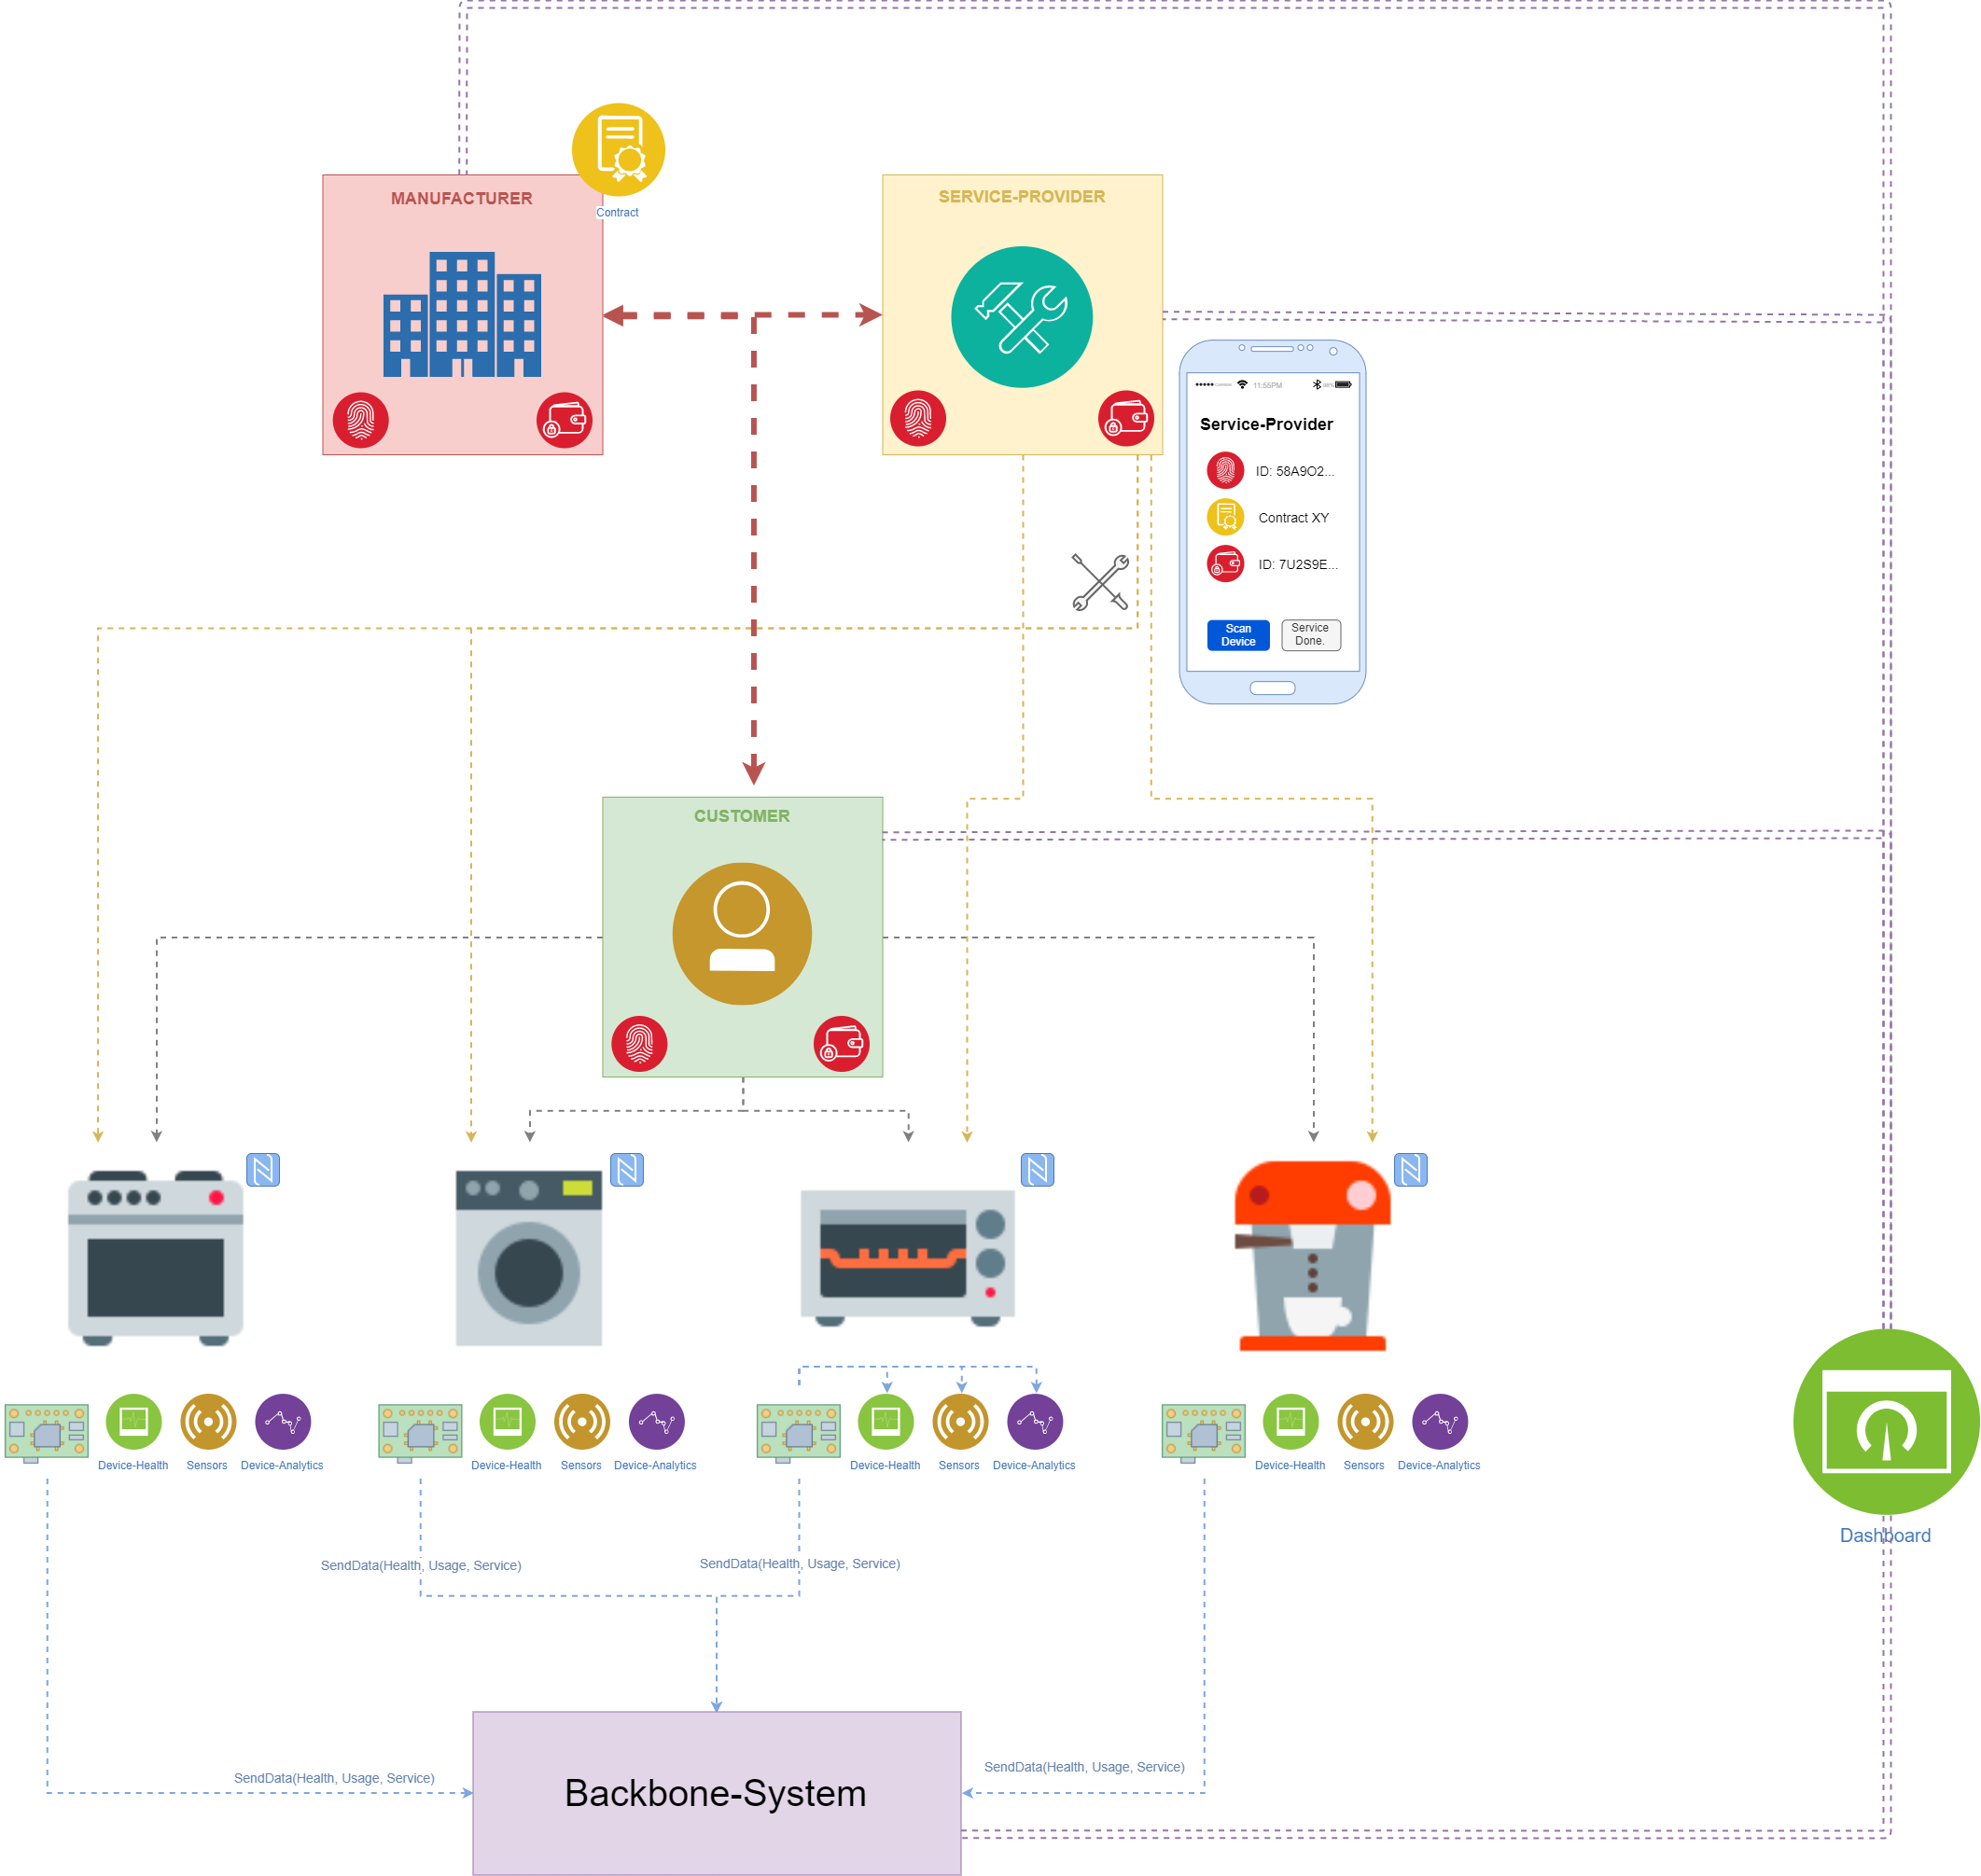
\includegraphics[width=1.0\textwidth]{gfx/IOT-Anwendungsfall.png}
 \caption{Grafische Veranschaulichung des Anwendungsfalls}
 \label{fig:chapter04:usecase}
\end{figure}


%
% Section: Beschreibung
%
\section{Beschreibung}
\label{sec:iot_usecase:description}
\lipsum[1-1]

%
% Section: Technische Lösungsskizze
%
\section{Technische Lösungsskizze}
\label{sec:iot_usecase:solution}
\lipsum[1-1]
